\ignore{
\begin{frame}
\frametitle{ImageNet}

\begin{center}
%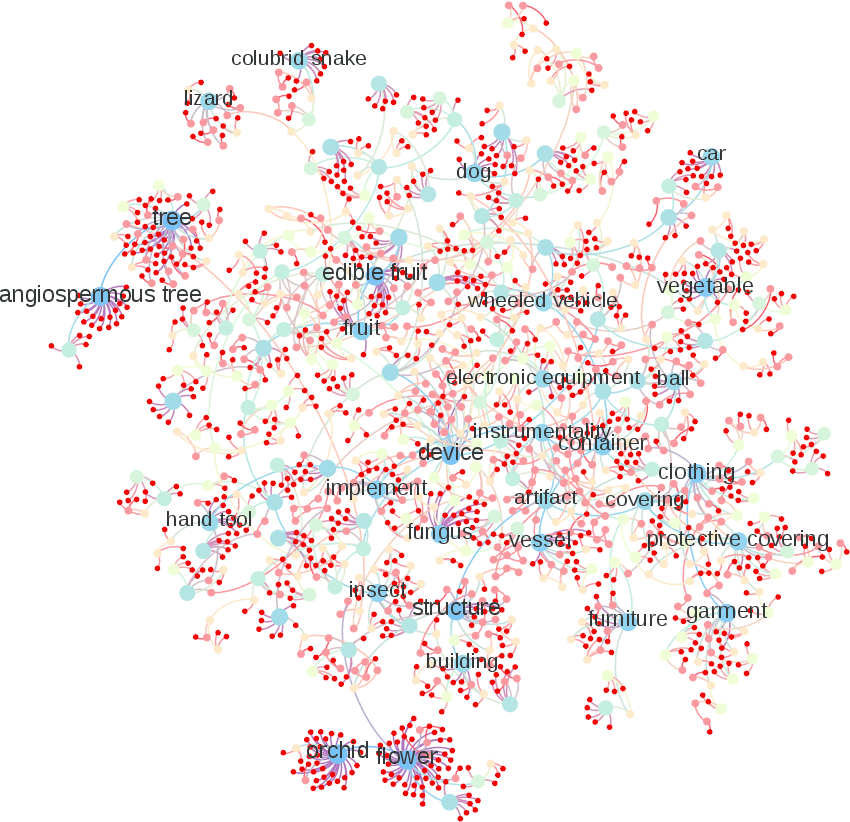
\includegraphics[height=2.7in]{img/imagenet-hierarchy}
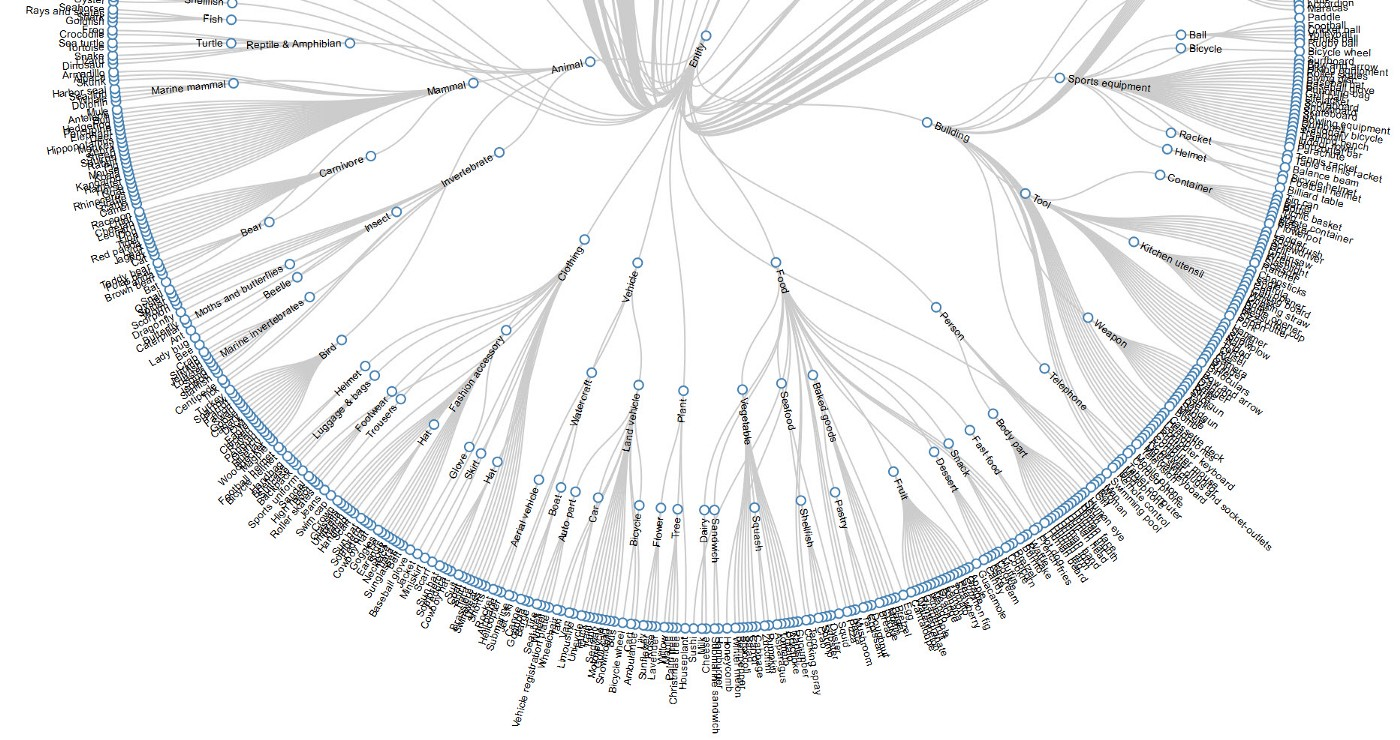
\includegraphics[width=\textwidth]{img/dendrogram}
\end{center}

1000 classes, hierarchically structured, 80 breeds of dog

{\tiny Image source: \citet{akata2014contributions}}
\end{frame}

%%%%%%%%%%%%%%%%%%%%%%%%%%%%%%%%%%%%%%%%

\begin{frame}
\frametitle{ImageNet}

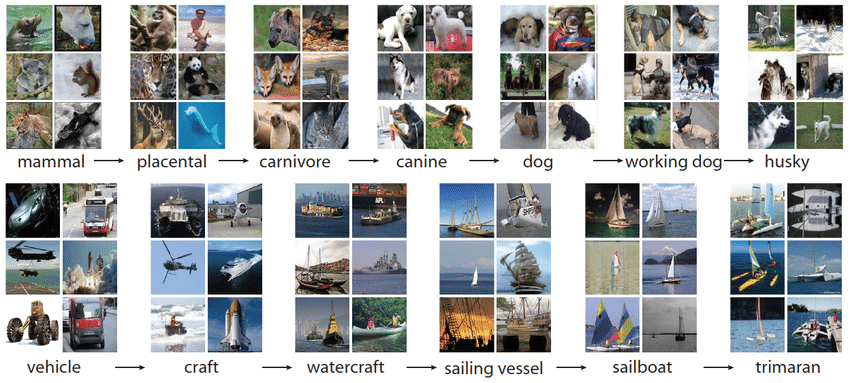
\includegraphics[width=\textwidth]{img/dog-trimaran}

{\tiny Image source: \citet{deng2012large}}
\end{frame}
}

%%%%%%%%%%%%%%%%%%%%%%%%%%%%%%%%%%%%%%%%

\begin{frame}
\frametitle{Real world data has lots of structure}

%ImageNet
%\begin{itemize}
%\item Most important image dataset
%\item 1.2 million images
%\item 1000 classes
%\item hierarchically structured
%\item 80 breeds of dog
%\end{itemize}
ImageNet has 1000 classes, hierarchical (DAG) class structure:

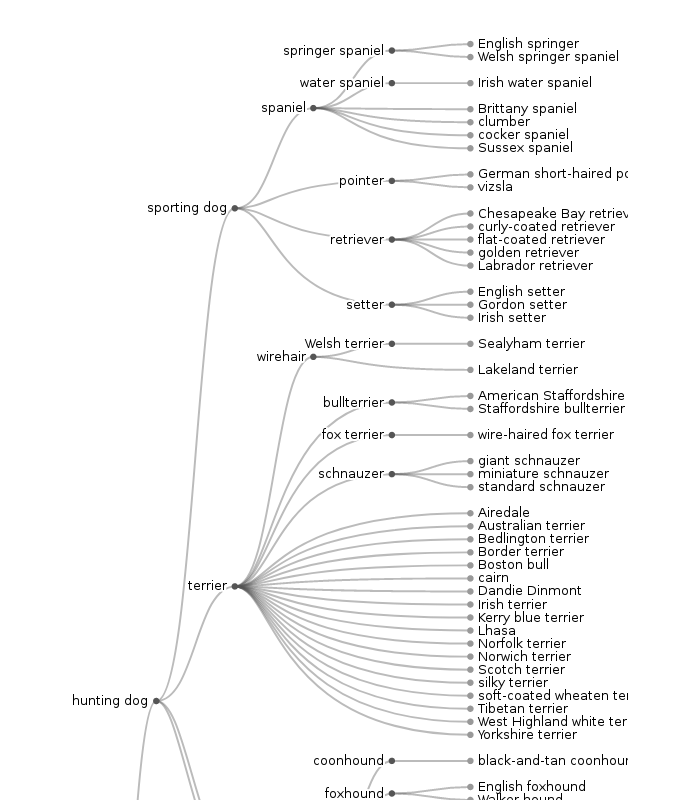
\includegraphics[height=2in]{img/imagent-hierarchy}

\vspace{0.25in}
Browse the hierarchy
\begin{itemize}
\item
\url{https://observablehq.com/@mbostock/imagenet-hierarchy}
\end{itemize}

\end{frame}

%%%%%%%%%%%%%%%%%%%%%%%%%%%%%%%%%%%%%%%%

\begin{frame}
\frametitle{Visualize this structure many ways}

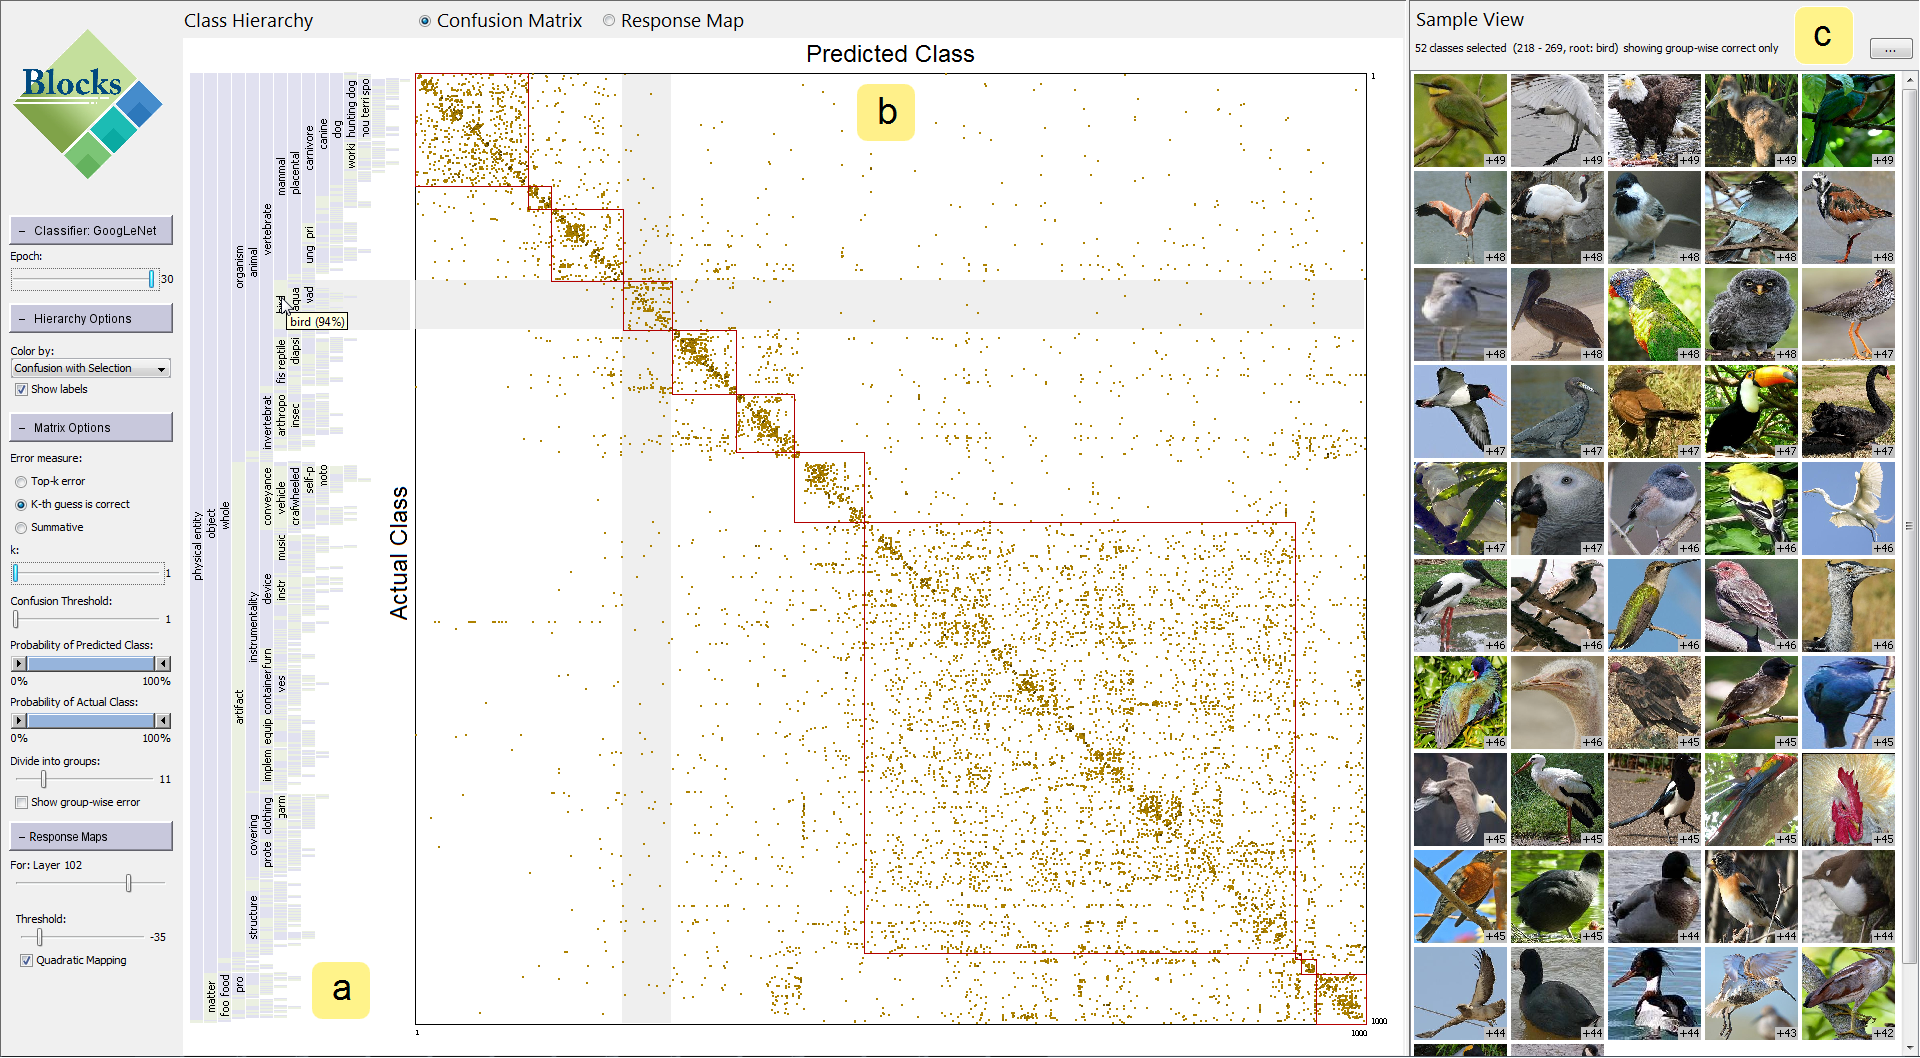
\includegraphics[width=\textwidth]{img/teaser}

{\tiny Image source: \citet{bilal2018}}
\end{frame}

